\documentclass[10pt]{article}
\usepackage[english]{babel}
\usepackage{../../../../lib/tex/naproche}
\usepackage{amssymb}
\usepackage{mathtools} % for \coloneq

\usepackage{stex-highlighting}
\providebool{emph} % "\newbool{emph}" does not work...
\setbool{emph}{false}
\colorlet{emphcolor}{violet}
\let\oldemph\emph
\renewcommand\emph[1]{\setbool{emph}{true}\ifbool{forthel}{\textcolor{emphcolor}{\itshape#1}}{\oldemph{#1}}\setbool{emph}{false}}
\renewcommand{\varemph}[1]{\ifbool{emph}{\textcolor{emphcolor}{#1}}{\textcolor{black}{#1}}}

\usepackage[right=6cm,left=3cm,bottom=3cm,marginparwidth=5cm]{geometry}

\usepackage{fancyhdr}
\renewcommand{\sectionmark}[1]{\markboth{#1}{}} 
\def\libarchive{}
\pagestyle{fancy}
\fancyhead[L]{\libarchive}
\fancyhead[C]{\nouppercase\leftmark}  % section title
\fancyhead[R]{\thepage}               % page number
\fancyfoot[C]{}                       % No page number in footer

\usepackage[nobottomtitles]{titlesec}
\titlespacing*{\section}{0pt}{30pt}{0pt}
\titlespacing*{\subsection}{0pt}{30pt}{0pt}
\titlespacing*{\subsubsection}{0pt}{30pt}{0pt}

\documentclass[12pt,oneside]{book}

\usepackage[foundations]{../../lib/tex/naproche}
\usepackage{../../lib/tex/libraries}
\usepackage{graphicx}
\usepackage{float}
\usepackage{caption}
\usepackage{footnote}

\makesavenoteenv{tabular} % Make footnotes work in tabular environments


\title{Foundations of Mathematics}
\author{Marcel Schütz}
\date{2022}

\begin{document}
  \maketitle

  \tableofcontents

  \begin{figure}[H]
    \centering
    \fbox{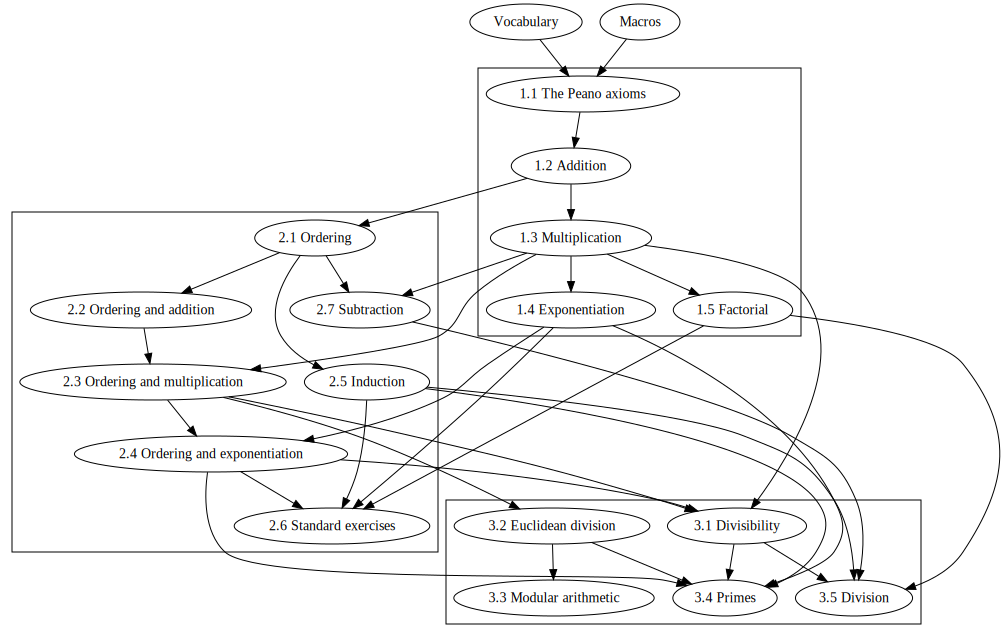
\includegraphics[width=0.9\linewidth]{./dependency-graph/graph.png}}
    \caption*{Interdependencies of the chapters}
  \end{figure}


  \section*{Introduction}

  This is a library providing a foundation of mathematics based on a
  Kelley-Morse like class theory with urelements.
  It introduces common operations on classes like unions or intersections
  (\cref{chapter:classes}) together with detailed proofs of their algebraic
  properties (\cref{chapter:computation-laws-for-classes}), the symmetric
  difference of two classes (\cref{chapter:symmetric-difference}) and the
  notions of ordered pairs and Cartesian products
  (\cref{chapter:pairs-and-products}) as well as proofs of the algebraic
  properties of the latter (\cref{chapter:computation-laws-for-products}).
  Moreover, it provides common operations on maps (\cref{chapter:maps}), various
  properties of images and preimages (\cref{chapter:image-and-preimage}) and the
  notions of injectivity, surjectivity, bijectivity
  (\cref{chapter:injections-surjections-bijections}) and invertibility of maps
  (\cref{chapter:invertible-maps}).
  The library provides an axiom system characterizing sets (\cref{chapter:sets})
  and, furthermore, it covers the notions of binary relations
  (\cref{chapter:binary-relations}), fixed-points of subset preserving maps
  (\cref{chapter:fixed-points}), including and equinumerosity
  (\cref{chapter:equinumerosity}).

  As two famous results it includes the Knaster-Tarski fixed point theorem
  (\cref{FOUNDATIONS_12_8420450166112256}) and the Cantor-Schröder-Bernstein
  theorem (\cref{FOUNDATIONS_13_1913663275401216}).

  \paragraph*{Usage.}
  At the very beginning of each chapter you can find the name of its source
  file, e.g. \path{foundations/sections/01_classes.ftl.tex} for
  \cref{chapter:classes}. This filename can be used to import the chapter via
  \Naproche's \texttt{readtex} instruction to another ForTheL text, e.g.:
  \begin{center}
    \verb`[readtex \path{foundations/sections/01_classes.ftl.tex}]`
  \end{center}

  \paragraph*{Checking times.}
  The checking times for each of the chapters may vary from computer to
  computer, but on mid-range hardware they are likely to be similar to those
  given in table below:

  \begin{center}
    \begin{tabular}{c|c|c}

      & \multicolumn{2}{c}{\textbf{Checking time}}
      \\
      \textbf{Chapter}
      & \textbf{without dependencies}     & \textbf{with dependencies}
      \\ \hline
      \ref{chapter:classes}
      & 00:04 min                         & 00:04 min
      \\
      \ref{chapter:computation-laws-for-classes}
      & 00:12 min                         & 00:16 min
      \\
      \ref{chapter:symmetric-difference}
      & 00:32 min                         & 00:48 min
      \\
      \ref{chapter:pairs-and-products}
      & 00:08 min                         & 00:12 min
      \\
      \ref{chapter:computation-laws-for-products}
      & 01:36 min                         & 01:56 min
      \\
      \ref{chapter:maps}
      & 01:13 min                         & 01:25 min
      \\
      \ref{chapter:image-and-preimage}
      & 01:28 min                         & 02:53 min
      \\
      \ref{chapter:injections-surjections-bijections}
      & 00:38 min                         & 02:03 min
      \\
      \ref{chapter:invertible-maps}
      & 02:20 min                         & 04:23 min
      \\
      \ref{chapter:sets}
      & 02:17 min                         & 06:40 min
      \\
      \ref{chapter:binary-relations}
      & 00:14 min                         & 06:54 min
      \\
      \ref{chapter:fixed-points}
      & 00:33 min                         & 07:13 min
      \\
      \ref{chapter:equinumerosity}
      & 01:48 min                         & 09:01 min
    \end{tabular}
  \end{center}


  \subfile{sections/01_classes.ftl.tex}
  \subfile{sections/02_computation-laws-for-classes.ftl.tex}
  \subfile{sections/03_symmetric-difference.ftl.tex}
  \subfile{sections/04_pairs-and-products.ftl.tex}
  \subfile{sections/05_computation-laws-for-products.ftl.tex}
  \subfile{sections/06_maps.ftl.tex}
  \subfile{sections/07_image-and-preimage.ftl.tex}
  \subfile{sections/08_injections-surjections-bijections.ftl.tex}
  \subfile{sections/09_invertible-maps.ftl.tex}
  \subfile{sections/10_sets.ftl.tex}
  \subfile{sections/11_binary-relations.ftl.tex}
  \subfile{sections/12_fixed-points.ftl.tex}
  \subfile{sections/13_equinumerosity.ftl.tex}
\end{document}

\begin{document}
  \begin{imports}
    \begin{forthel}
      %[prove off][check off]

      [readtex \path{libraries/source/foundations/09_invertible-maps.ftl.tex}]

      %[prove on][check on]
    \end{forthel}
  \end{imports}


  \section{Sub- and Supersets}

  \begin{forthel}
    \begin{definition}\printlabel{FOUNDATIONS_10_1346889551183872}
      Let $A$ be a class.
      A subset of $A$ is a subclass of $A$ that is a set.
    \end{definition}

    Let a superset of $A$ stand for a superclass of $A$ that is a set.
    Let a proper subset of $A$ stand for a proper subclass of $A$ that is a set.
    Let a proper superset of $A$ stand for a proper superclass of $A$ that is a
    set.
  \end{forthel}


  \section{Powerclasses}

  \begin{forthel}
    \begin{definition}\printlabel{FOUNDATIONS_10_1448589907722240}
      Let $A$ be a class.
      The powerclass of $A$ is
      \[ \{ x \mid \text{$x$ is a subset of $A$} \}. \]
    \end{definition}

    Let $\pow(A)$ stand for the powerclass of $A$.
  \end{forthel}


  \section{Systems of Sets}

  \begin{forthel}
    \begin{definition}\printlabel{FOUNDATIONS_10_5805323570905088}
      A system of sets is a class $X$ such that every element of $X$ is a set.
    \end{definition}
  \end{forthel}

  \begin{forthel}
    \begin{definition}\printlabel{FOUNDATIONS_10_1631952387964928}
      A system of nonempty sets is a class $X$ such that every element of $X$ is
      a nonempty set.
    \end{definition}
  \end{forthel}

  \begin{forthel}
    \begin{definition}\printlabel{FOUNDATIONS_10_943381479948288}
      Let $A$ be a class.
      A system of subsets of $A$ is a class $X$ such that every element of $X$
      is a subset of $A$.
    \end{definition}
  \end{forthel}

  \begin{forthel}
    \begin{definition}\printlabel{FOUNDATIONS_10_1394550966845440}
      A map between systems of sets is a map from some system of sets to some
      system of sets.
    \end{definition}
  \end{forthel}

  \begin{forthel}
    \begin{definition}\printlabel{FOUNDATIONS_10_3290499861446656}
      Let $f$ be a map between systems of sets.
      $f$ is subset preserving iff for all $x, y \in \dom(f)$
      \[ x \subseteq y \implies f(x) \subseteq f(y). \]
    \end{definition}

    Let $f$ preserves subsets stand for $f$ is subset preserving.
  \end{forthel}

  \begin{forthel}
    \begin{proposition}\printlabel{FOUNDATIONS_10_8268633648136192}
      Let $A$ be a class.
      Then $\emptyset$ is a system of subsets of $A$.
    \end{proposition}
  \end{forthel}

  \begin{forthel}
    \begin{proposition}\printlabel{FOUNDATIONS_10_7546016869908480}
      Let $A$ be a class.
      Then $\pow(A)$ is a system of subsets of $A$.
    \end{proposition}
  \end{forthel}

  \begin{forthel}
    \begin{proposition}
      Let $X, Y$ be systems of sets.
      Then $X \cup Y$ is a system of sets.
    \end{proposition}
  \end{forthel}

  \begin{forthel}
    \begin{proposition}
      Let $X, Y$ be systems of sets.
      Then $X \cap Y$ is a system of sets.
    \end{proposition}
  \end{forthel}

  \begin{forthel}
    \begin{proposition}
      Let $X, Y$ be systems of sets.
      Then $X \setminus Y$ is a system of sets.
    \end{proposition}
  \end{forthel}


  \section{Unions}

  \begin{forthel}
    \begin{definition}\printlabel{FOUNDATIONS_10_541772562300928}
      Let $X$ be a system of sets.
      The union over $X$ is
      \[ \{ a \mid \text{$a \in x$ for some $x \in X$} \}. \]
    \end{definition}

    Let $\bigcup X$ stand for the union over $X$.
  \end{forthel}

  \begin{forthel}
    \begin{proposition}\printlabel{FOUNDATIONS_10_4872701241982976}
      \[ \bigcup \emptyset = \emptyset. \]
    \end{proposition}
    \begin{proof}
      $\bigcup \emptyset = \{ a \mid a \in x$ for some $x \in \emptyset \}$.
      $\emptyset$ has no elements.
      Hence there is no object $a$ such that $a \in x$ for some
      $x \in \emptyset$.
      Thus $\bigcup \emptyset = \emptyset$.
    \end{proof}
  \end{forthel}

  \begin{forthel}
    \begin{proposition}\printlabel{FOUNDATIONS_10_2559541585641472}
      Let $x, y$ be sets.
      Then \[ \bigcup \set{x, y} = x \cup y. \]
    \end{proposition}
    \begin{proof}
      Let us show that $\bigcup \set{x, y} \subseteq x \cup y$.
        Let $a \in \bigcup \set{x, y}$.
        Then $a$ is contained in some element of $\set{x, y}$.
        Hence $a \in x$ or $a \in y$.
        Thus $a \in x \cup y$.
      End.

      Let us show that $x \cup y \subseteq \bigcup \set{x, y}$.
        Let $a \in x \cup y$.
        Then $a \in x$ or $a \in y$.
        Hence $a$ is contained in some element of $\set{x, y}$.
        Therefore $a \in \bigcup \set{x, y}$.
      End.
    \end{proof}
  \end{forthel}

  \begin{forthel}
    \begin{corollary}\printlabel{FOUNDATIONS_10_2157223832715264}
      Let $x$ be a set.
      Then \[ \bigcup \set{x} = x. \]
    \end{corollary}
  \end{forthel}


  \section{Intersections}

  \begin{forthel}
    \begin{definition}\printlabel{FOUNDATIONS_10_2659345095458816}
      Let $X$ be a system of sets.
      The intersection over $X$ is
      \[ \{ a \mid \text{$a \in x$ for all $x \in X$} \}. \]
    \end{definition}

    Let $\bigcap X$ stand for the intersection over $X$.
  \end{forthel}

  \begin{forthel}
    \begin{proposition}\printlabel{FOUNDATIONS_10_2809770322952192}
      $\bigcap \emptyset$ is the class of all objects.
    \end{proposition}
    \begin{proof}
      Define $V = \{ x \mid x$ is an object $\}$.
      We have $\bigcap \emptyset \subseteq V$.
      Indeed every element of $\bigcap \emptyset$ is an object.

      Let us show that $V \subseteq \bigcap \emptyset$.
        Let $a \in V$.
        Then $a$ is an object.
        For every $x \in \emptyset$ we have $a \in x$.
        Indeed $\emptyset$ has no elements.
        Thus $a \in \bigcap \emptyset$.
      End.
    \end{proof}
  \end{forthel}

  \begin{forthel}
    \begin{proposition}\printlabel{FOUNDATIONS_10_7851827447988224}
      Let $x, y$ be sets.
      Then \[ \bigcap \set{x, y} = x \cap y. \]
    \end{proposition}
    \begin{proof}
      Let us show that $\bigcap \set{x, y} \subseteq x \cap y$.
        Let $a \in \bigcap \set{x, y}$.
        Then $a$ is contained in every element of $\set{x, y}$.
        Hence $a \in x$ and $a \in y$.
        Thus $a \in x \cap y$.
      End.

      Let us show that $x \cap y \subseteq \bigcap \set{x, y}$.
        Let $a \in x \cap y$.
        Then $a \in x$ and $a \in y$.
        Hence $a$ is contained in every element of $\set{x, y}$.
        Therefore $a \in \bigcap \set{x, y}$.
      End.
    \end{proof}
  \end{forthel}

  \begin{forthel}
    \begin{corollary}\printlabel{FOUNDATIONS_10_7239895674257408}
      Let $x$ be a set.
      Then \[ \bigcap \set{x} = x. \]
    \end{corollary}
  \end{forthel}
\end{document}
